\chapter{Implementing a maximum volume fraction in the slip model}\label{appendixc}

Attempts were made to implement a maximum volume fraction $\alpha_{max}$ into equation \ref{eq:coalescencebarrier} and \ref{eq:bubbly5}, equation \ref{eq:bubbly5} can be rearranged as:

\begin{equation}
    \mu = \frac{\mu_c}{1-\alpha_d/\alpha_{max}}
\end{equation}

It is found that this implementation could only slightly suppress the volume fraction, as shown in figure \ref{04phim}, and \ref{038phim}.


\begin{figure}[H]
    \centering
    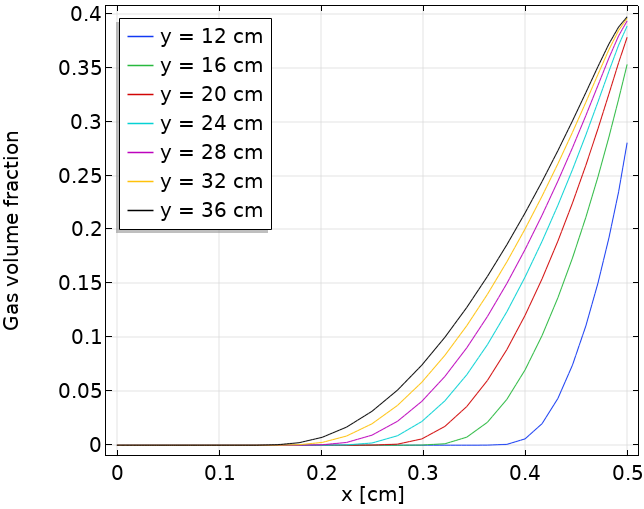
\includegraphics[width=0.8\textwidth]{maxphi042000A.png}
    \caption{$\alpha_{max}=0.4$, $i_{av}=2000 \, \mathrm{A/m^2}$, the simulation was done in a similar setup with the one introduced in chapter 4, only the riser channel is $30 \, \mathrm{cm}$ tall instead of $30 \, \mathrm{cm}$}
    \label{04phim}
\end{figure}

\begin{figure}[H]
    \centering
    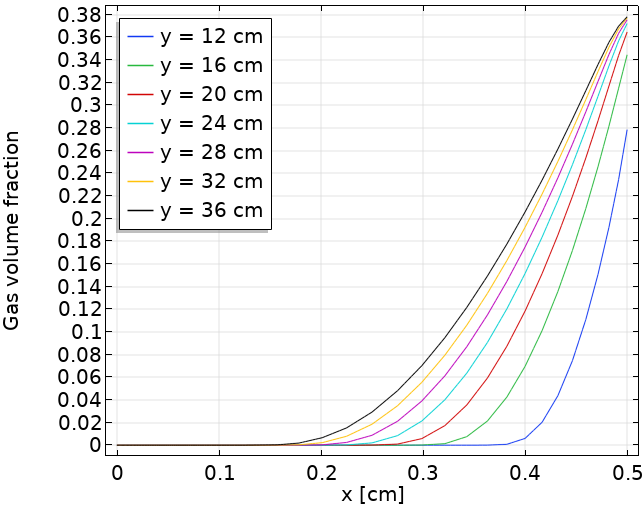
\includegraphics[width=0.8\textwidth]{maxphi0381000A.png}
    \caption{$\alpha_{max}=0.38$, $i_{av}=1000 \, \mathrm{A/m^2}$,the simulation was done in a similar setup with the one introduced in chapter 4, only the riser channel is $30 \, \mathrm{cm}$ tall instead of $30 \, \mathrm{cm}$}
    \label{038phim}
\end{figure}

When the input current density increases, the $\alpha_{max}$ has to increase as well, or the solver will crash.